As part of the design guidelines for Google Glass, Google provides developers with a card layout template, seen in Figure~\ref{GlassDesignStyle}. The different coloured regions are intended for different types of information. The red area is the main area intended for presenting information in text form with the green squares representing the preferred margins. The thick blue stripe almost at the bottom marks the footer. The footer should hold supplementary information, such as a user name or a timestamp. The blue,  slightly transparent, area to the left is mainly intended for images with associated text being presented to the right. The grey area, seemingly appearing behind all the other coloured areas, represent the entire card, with a size of 640 pixels wide and 360 pixels high~\cite{glassDesignStyle}.

	\begin{figure}[ht!]
		\centering
		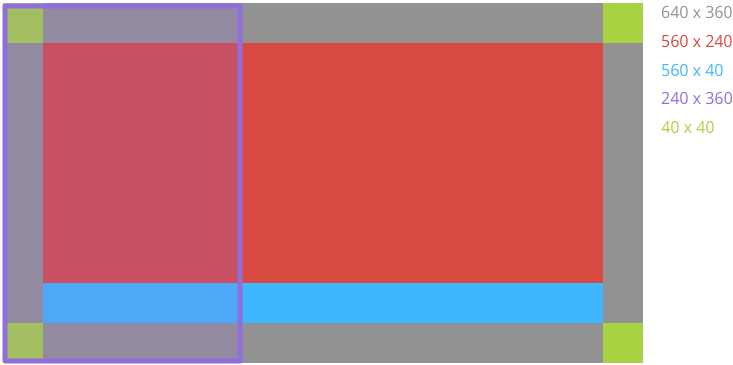
\includegraphics[width=110mm]{images/standard-template}
		\caption{Google's design guidelines include a card layout template~\cite{glassDesignStyle}.}
		\label{GlassDesignStyle}
	\end{figure}

Google goes even further in providing developers with guidelines for the design of cards. Google provides developers with a set of fixed card layouts. Specific card layouts set up the necessary margins and leave the developers to input the information to be displayed. Four examples of fixed card layouts can be seen in Figure~\ref{cardLayouts}.

	\begin{figure}[ht!]
		\centering
   		\subfloat[Text layout.]{{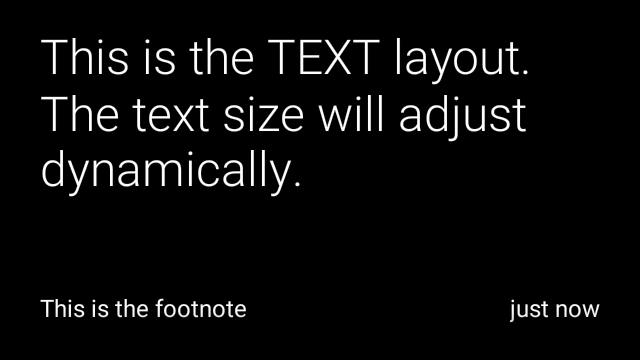
\includegraphics[width=70mm]{images/card_text} }}
  	 \qquad
   		\subfloat[Fixed text layout.]{{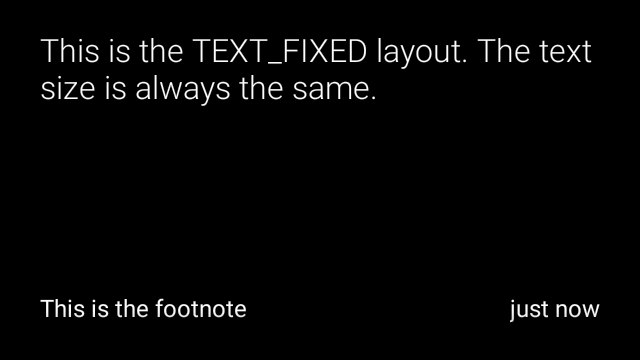
\includegraphics[width=70mm]{images/card_text_fixed} }}
	\qquad
		\subfloat[Columns layout.]{{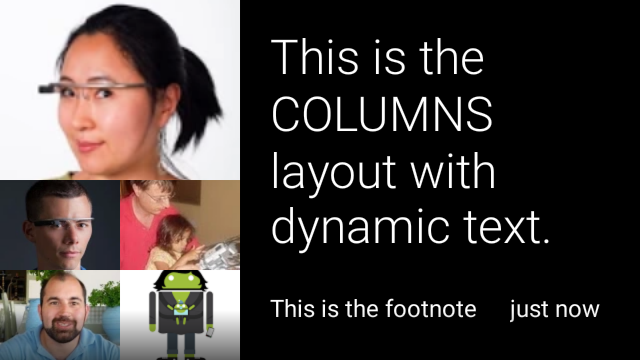
\includegraphics[width=70mm]{images/card_columns} }}
   	\qquad
		\subfloat[Title layout.]{{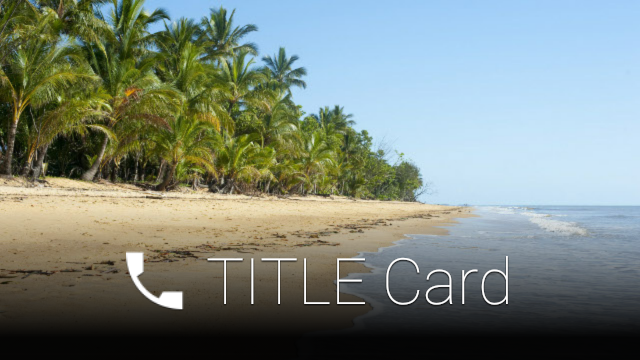
\includegraphics[width=70mm]{images/card_title} }}
   	\qquad
		\caption{Four different standard card layouts~\cite{cardLayout}.}
		\label{cardLayouts}
	\end{figure}

In terms of the information displayed, Google's default typeface family is called ``Roboto''. Google states that Roboto's geometrical forms and open curves makes for a natural reading rhythm~\cite{googleTypefaceRoboto}. Roboto is the typeface family used on all of Google's standard card layouts, some of which are seen in Figure~\ref{cardLayouts}. Google uses different typfaces from the Roboto typeface family for different texts~\cite{glassDesignStyle}. Roboto Light is most common, with Roboto Regular being used for footnote text and Roboto Thin being used for larger texts, such as titles on the title card layout seen in Figure~\ref{cardLayouts}~(d).

One of the advantages of using Google's default layout is the fact that the text is dynamically resized to fit the card. Dynamically resized text means that the text is only as small as the text needs to be. However, there is a minimum size text may be downsized to. At 32 pixels the text is as small as the text may be and any text that does not fit on the card at that point is truncated.

Due to the limitation on the amount of text that may be presented on screen at the same time Google have provided developers with guidelines on how to present written information on Google Glass~\cite{glassDesignStyle}. The guidelines for writing are five in total and read as follows:

\begin{itemize}
	\item \textbf{Keep it brief.} Be concise, simple and precise. Look for alternatives to long text such as reading the content aloud, showing images or video, or removing features.
	\item \textbf{Keep it simple.} Pretend you're speaking to someone who's smart and competent, but doesn't know technical jargon and may not speak English very well. Use short words, active verbs, and common nouns.
	\item \textbf{Be friendly.} Use contractions. Talk directly to the reader using second person (``you''). If your text doesn't read the way you'd say it in casual conversation, it's probably not the way you should write it.
	\item \textbf{Put the most important thing first.} The first two words (around 11 characters, including spaces) should include at least a taste of the most important information in the string. If they don't, start over. Describe only what's necessary, and no more. Don't try to explain subtle differences. They will be lost on most users.
	\item \textbf{Avoid repetition.} If a significant term gets repeated within a screen or block of text, find a way to use it just once.
\end{itemize}

Another part of Google Glass applications where Google have provided guidelines is voice commands~\cite{googleGlassVoiceCommand}. However, voice commands might be the most restrictive area of all in terms of what Google recommend developers to do. Any voice command not officially approved by Google is not allowed in an application if the application is to be released on MyGlass. MyGlass is the official store from which users may buy their Google Glass applications. However, MyGlass is not installed on Google Glass but rather on, for instance, a smartphone~\cite{myGlass}.

Only by using the approved main voice commands~\cite{existingVoiceCommands} will applications be approved and allowed on MyGlass. These approved main voice commands does not, however, include for instance ``next slide''. Unapproved voice commands may be used during development and for separate releases. Developers may also use the built-in speech recognition. However, using speech recognition would mean not being able to launch the voice recognition simply saying ``ok glass'', which is the case with approved and unapproved voice commands.

In terms of getting a voice command approved, Google have set up a checklist for developers to cross off as they design their voice commands~\cite{glassVoiceChecklist}. The checklist includes not designing a voice command which is similar to an already existing voice command. The voice command should also be long enough to ensure high recognition quality, yet short enough to fit on a single line on the Google Glass display.